\documentclass{article}

\usepackage[
  paperwidth=200mm,
  paperheight=55mm,
  margin=0mm
]{geometry}

\usepackage{tikz}
\usepackage{amsmath}
\usepackage{sfmath}
\usepackage{adjustbox}
\usetikzlibrary{arrows.meta,calc}

\pagestyle{empty}
\setlength{\parindent}{0pt}

\begin{document}

\hspace*{10mm}%
\begin{adjustbox}{
    max width=188mm,
    max height=53mm,
    keepaspectratio
  }

  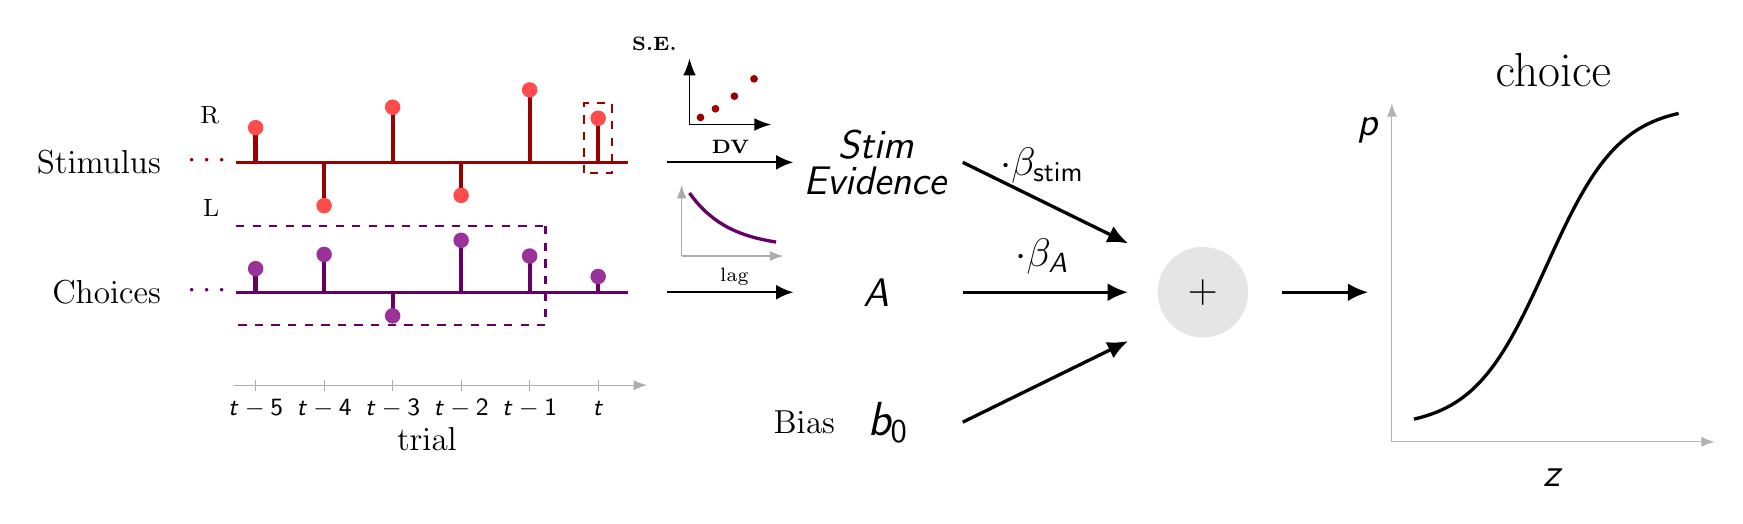
\begin{tikzpicture}[
      font=\sffamily,
      >=Latex,
      arrow/.style={
        very thick,
        -{Latex[length=2.6mm,width=2.3mm]}
      },
      smallarrow/.style={
        thick,
        -{Latex[length=2.2mm,width=1.9mm]}
      },
      sum/.style={
        circle,
        minimum size=1.15cm,
        fill=gray!20,
        draw=none,
        font=\Large
      }
    ]

    % =====================================================
    % GLOBAL GEOMETRY
    % =====================================================

    \def\yStim{1.65}
    \def\yHist{0.00}
    \def\yBias{-1.65}

    % =====================================================
    % TEMPORAL BLOCK
    % =====================================================

    \def\xWeightsC{5.10}
    \def\trialStep{0.87}
    \def\xTrialStart{\xWeightsC-2.18}

    \pgfmathsetmacro{\xTrialEnd}
    {\xTrialStart+5*\trialStep+0.38}

    % =====================================================
    % INTERMEDIATE ARROWS / REGRESSOR LABELS
    % =====================================================

    \def\xSmallArrowStart{8.15}
    \def\xSmallArrowEnd{9.75}

    % =====================================================
    % SCHEMATIC COLUMN
    % =====================================================

    \def\xRegC{10.80}

    % =====================================================
    % GLM BLOCK
    % =====================================================

    \def\xModelStart{11.90}
    \def\xSigma{14.95}
    \def\xPsych{17.35}

    % =====================================================
    % ROW LABELS
    % =====================================================

    \node[
      font=\large,
      anchor=east
    ]
    at (\xTrialStart-1.08,\yStim)
    {Stimulus};

    \node[
      font=\large,
      anchor=east
    ]
    at (\xTrialStart-1.08,\yHist)
    {Choices};

    % =====================================================
    % STIMULUS LEADING DOTS
    % =====================================================

    \node[
      red!60!black,
      font=\large
    ]
    at (\xTrialStart-0.58,\yStim+0.02)
    {$\cdots$};

    % =====================================================
    % STIMULUS BASELINE
    % =====================================================

    \draw[
      red!60!black,
      line width=1.25pt
    ]
    (\xTrialStart-0.25,\yStim)
    --
    (\xTrialEnd,\yStim);

    % =====================================================
    % STIMULUS WEIGHTS
    % =====================================================

    \foreach \i/\h in {
      0/0.44,
      1/-0.55,
      2/0.70,
      3/-0.42,
      4/0.92,
      5/0.56
    }{
      \pgfmathsetmacro{\x}
      {\xTrialStart+\trialStep*\i}

      \draw[
        red!60!black,
        line width=1.55pt
      ]
      (\x,\yStim)
      --
      (\x,\yStim+\h);

      \fill[
        red!70
      ]
      (\x,\yStim+\h)
      circle (2.8pt);
    }

    % R / L
    \node[
      font=\small,
      anchor=east
    ]
    at (\xTrialStart-0.34,\yStim+0.60)
    {R};

    \node[
      font=\small,
      anchor=east
    ]
    at (\xTrialStart-0.34,\yStim-0.58)
    {L};

    % =====================================================
    % SELECTED CURRENT STIMULUS
    % =====================================================

    \pgfmathsetmacro{\xStimSelected}
    {\xTrialStart+5*\trialStep}

    \draw[
      dashed,
      thick,
      red!60!black
    ]
    (\xStimSelected-0.18,\yStim-0.14)
    rectangle
    (\xStimSelected+0.18,\yStim+0.75);

    % =====================================================
    % HISTORY LEADING DOTS
    % =====================================================

    \node[
      violet!80!black,
      font=\large
    ]
    at (\xTrialStart-0.58,\yHist+0.02)
    {$\cdots$};

    % =====================================================
    % HISTORY BASELINE
    % =====================================================

    \draw[
      violet!80!black,
      line width=1.25pt
    ]
    (\xTrialStart-0.25,\yHist)
    --
    (\xTrialEnd,\yHist);

    % =====================================================
    % HISTORY WEIGHTS
    % =====================================================

    \foreach \i/\h in {
      0/0.30,
      1/0.48,
      2/-0.30,
      3/0.66,
      4/0.46,
      5/0.20
    }{
      \pgfmathsetmacro{\x}
      {\xTrialStart+\trialStep*\i}

      \draw[
        violet!80!black,
        line width=1.55pt
      ]
      (\x,\yHist)
      --
      (\x,\yHist+\h);

      \fill[
        violet!80
      ]
      (\x,\yHist+\h)
      circle (2.8pt);
    }

    % =====================================================
    % HISTORY SELECTION — OPEN ON LEFT
    % =====================================================

    \pgfmathsetmacro{\xHistSelStart}
    {\xTrialStart-0.25}

    \pgfmathsetmacro{\xHistSelEnd}
    {\xTrialStart+4*\trialStep+0.20}

    \pgfmathsetmacro{\yHistSelBottom}
    {\yHist-0.42}

    \pgfmathsetmacro{\yHistSelTop}
    {\yHist+0.84}

    \draw[
      dashed,
      thick,
      violet!80!black
    ]
    (\xHistSelStart,\yHistSelTop)
    --
    (\xHistSelEnd,\yHistSelTop);

    \draw[
      dashed,
      thick,
      violet!80!black
    ]
    (\xHistSelEnd,\yHistSelTop)
    --
    (\xHistSelEnd,\yHistSelBottom);

    \draw[
      dashed,
      thick,
      violet!80!black
    ]
    (\xHistSelEnd,\yHistSelBottom)
    --
    (\xHistSelStart,\yHistSelBottom);

    % =====================================================
    % TRIAL AXIS
    % =====================================================

    \def\yTrialAxis{-1.18}

    \draw[
      gray!65,
      ->
    ]
    (\xTrialStart-0.28,\yTrialAxis)
    --
    (\xTrialStart+5*\trialStep+0.62,\yTrialAxis);

    \foreach \i/\lab in {
      0/$t-5$,
      1/$t-4$,
      2/$t-3$,
      3/$t-2$,
      4/$t-1$,
      5/$t$
    }{
      \pgfmathsetmacro{\x}
      {\xTrialStart+\trialStep*\i}

      \draw[
        gray!65
      ]
      (\x,\yTrialAxis+0.07)
      --
      (\x,\yTrialAxis-0.07);

      \node[
        font=\small
      ]
      at (\x,\yTrialAxis-0.30)
      {\lab};
    }

    \node[
      font=\large
    ]
    at (
      {\xTrialStart+2.5*\trialStep},
      {\yTrialAxis-0.68}
    )
    {trial};

    % =====================================================
    % INTERMEDIATE ARROWS
    % =====================================================

    % Stimulus arrow
    \draw[
      smallarrow
    ]
    (\xSmallArrowStart,\yStim)
    --
    (\xSmallArrowEnd,\yStim);

    % Choices arrow
    \draw[
      smallarrow
    ]
    (\xSmallArrowStart,\yHist)
    --
    (\xSmallArrowEnd,\yHist);

    % Regressor names after the arrows
    \node[
      font=\Large,
      align=center
    ]
    at (\xRegC,\yStim)
    {\shortstack{$Stim$\\$Evidence$}};

    \node[
      font=\Large
    ]
    at (\xRegC,\yHist)
    {$A$};

    % =====================================================
    % SCHEMATICS ABOVE THE ARROWS
    % =====================================================

    % -----------------------------------------------------
    % STIMULUS EVIDENCE SCHEMATIC
    % First quadrant only
    % y label = S.E.
    % x label = DV
    % -----------------------------------------------------

    \def\xStimScheme{8.95}
    \def\yStimScheme{2.55}

    % First-quadrant axes:
    % the origin is placed at the lower-left corner
    \draw[
      black,
      line width=0.7pt,
      ->
    ]
    (\xStimScheme-0.52,\yStimScheme-0.42)
    --
    (\xStimScheme+0.52,\yStimScheme-0.42);

    \draw[
      black,
      line width=0.7pt,
      ->
    ]
    (\xStimScheme-0.52,\yStimScheme-0.42)
    --
    (\xStimScheme-0.52,\yStimScheme+0.42);

    % Positive points only
    \foreach \dx/\dy in {
      0.14/0.09,
      0.33/0.20,
      0.57/0.36,
      0.82/0.58
    }{
      \fill[
        red!60!black
      ]
      (
        {\xStimScheme-0.52+\dx},
        {\yStimScheme-0.42+\dy}
      )
      circle (1.4pt);
    }

    % S.E. label remains unchanged in this diagram
    \node[
      font=\scriptsize\bfseries,
      anchor=south east
    ]
    at (\xStimScheme-0.56,\yStimScheme+0.40)
    {S.E.};

    \node[
      font=\scriptsize\bfseries,
      anchor=north
    ]
    at (\xStimScheme,\yStimScheme-0.49)
    {DV};

    % -----------------------------------------------------
    % ACTION TRACE / EXPONENTIAL DECAY
    % -----------------------------------------------------

    \def\xHistScheme{8.95}
    \def\yHistScheme{0.88}

    % axes
    \draw[
      gray!65,
      ->
    ]
    (\xHistScheme-0.62,\yHistScheme-0.42)
    --
    (\xHistScheme+0.67,\yHistScheme-0.42);

    \draw[
      gray!65,
      ->
    ]
    (\xHistScheme-0.62,\yHistScheme-0.42)
    --
    (\xHistScheme-0.62,\yHistScheme+0.48);

    % exponential decay
    \draw[
      violet!80!black,
      very thick,
      domain=0:1.10,
      samples=80
    ]
    plot (
      {\xHistScheme-0.52+\x},
      {\yHistScheme-0.32+0.70*exp(-2.0*\x)}
    );

    % x label = lag
    \node[
      font=\scriptsize
    ]
    at (\xHistScheme+0.05,\yHistScheme-0.68)
    {lag};

    % =====================================================
    % BIAS
    % =====================================================

    \node[
      font=\large,
      anchor=east
    ]
    at (\xRegC-0.40,\yBias)
    {Bias};

    \node[
      font=\LARGE
    ]
    at (\xRegC+0.15,\yBias)
    {$b_0$};

    % =====================================================
    % SUM
    % =====================================================

    \node[
      sum
    ] (sum)
    at (\xSigma,0)
    {$+$};

    % =====================================================
    % MODEL ARROWS
    % =====================================================

    % -----------------------------------------------------
    % STIMULUS
    % -----------------------------------------------------

    \coordinate (stimStart)
    at (\xModelStart,\yStim);

    \coordinate (stimEnd)
    at (\xSigma-0.95,0.62);

    \draw[arrow]
    (stimStart)
    --
    (stimEnd);

    \path
    (stimStart) -- (stimEnd)
    coordinate[pos=0.48] (stimBetaPos);

    \node[
      font=\Large,
      yshift=13pt
    ]
    at (stimBetaPos)
    {$\cdot\beta_{\rm stim}$};

    % -----------------------------------------------------
    % HISTORY
    % -----------------------------------------------------

    \coordinate (histStart)
    at (\xModelStart,\yHist);

    \coordinate (histEnd)
    at (\xSigma-0.95,0);

    \draw[arrow]
    (histStart)
    --
    (histEnd);

    \path
    (histStart) -- (histEnd)
    coordinate[pos=0.48] (histBetaPos);

    \node[
      font=\Large,
      yshift=13pt
    ]
    at (histBetaPos)
    {$\cdot\beta_A$};

    % -----------------------------------------------------
    % BIAS
    % -----------------------------------------------------

    \coordinate (biasStart)
    at (\xModelStart,\yBias);

    \coordinate (biasEnd)
    at (\xSigma-0.95,-0.62);

    \draw[arrow]
    (biasStart)
    --
    (biasEnd);

    % =====================================================
    % SUM -> SIGMOID
    % =====================================================

    \draw[arrow]
    (\xSigma+1,0)
    --
    (\xPsych-0.30,0);

    % =====================================================
    % LARGE SIGMOID
    % =====================================================

    \def\sigW{4.10}
    \def\sigH{4.10}

    \draw[
      gray!60,
      ->
    ]
    (\xPsych,-1.90)
    --
    (\xPsych+\sigW,-1.90);

    \draw[
      gray!60,
      ->
    ]
    (\xPsych,-1.90)
    --
    (\xPsych,2.40);

    \def\sigmoid(#1){1/(1+exp(-#1))}

    \draw[
      very thick,
      domain=-3.6:3.6,
      samples=120
    ]
    plot (
      {\xPsych+0.28+\sigW*0.82*(\x+3.6)/7.2},
      {-1.72+\sigH*\sigmoid(\x)}
    );

    \node[
      font=\Large
    ]
    at (\xPsych-0.30,2.05)
    {$p$};

    \node[
      font=\Large
    ]
    at (\xPsych+2.05,-2.35)
    {$z$};

    \node[
      font=\LARGE
    ]
    at (\xPsych+2.05,2.82)
    {choice};

  \end{tikzpicture}

\end{adjustbox}

\end{document}